%
\documentclass[referee]{aa} % for a referee version
%\documentclass[onecolumn]{aa} % for a paper on 1 column  
%\documentclass[longauth]{aa} % for the long lists of affiliations 
%\documentclass[letter]{aa} % for the letters 
%\documentclass[bibyear]{aa} % if the references are not structured 
%                              according to the author-year natbib style


%\documentclass{aa}  

\usepackage{graphicx}
%%%%%%%%%%%%%%%%%%%%%%%%%%%%%%%%%%%%%%%%
\usepackage{txfonts}
\usepackage{multirow}
%%%%%%%%%%%%%%%%%%%%%%%%%%%%%%%%%%%%%%%%
\usepackage{subcaption}

  % results heading (mandatory)
\begin{document} 


   \title{Data processing pipelines and the data center for the X-ray spectrometer/imager STIX}

   \subtitle{}

   \author{Hualin Xiao
          \inst{1}
          \and 
          Shane Maloney 
          \inst{2}
          \and 
          Ewan Dickson \inst{4}
          \and 
          S\"am Krucker\inst{1}
          \and Andrea Francesco Battaglia\inst{3}
            \and László Etesi \inst{1}
          \and Ryan Daniel \inst{1}
          \and Lastufka Erica \inst{1}
          \and Olivier Limousin \inst{5}
          \and Nicky Hochmuth \inst{1}
          \and Other STIX team members
         }

   \institute{University of Applied Sciences and Arts Northwestern Switzerland (FHNW), 5200 Windisch, Switzerland \\
              \email{hualin.xiao@fhnw.ch}
         \and
          Astrophysics Research Group, School of Physics, Trinity College Dublin, Dublin 2, Ireland
          \and
             ETH Z\"urich, R\"amistrasse 101, 8092 Z\"urich, Switzerland
         \and University of Graz, Universitätspl. 3, 8010 Graz, Austria
         \and IRFU, CEA, Université Paris-Saclay, and Université Paris Diderot, AIM, Sorbonne Paris Cité, CEA, CNRS, 91191 Gif-sur-Yvette,
         France
             }

   \date{}

% \abstract{}{}{}{}{} 
% 5 {} token are mandatory
 
  \abstract
  % context heading (optional)
   {} %leave it empty if necessary  
  % {context.}
  % aims heading (mandatory)
   { The Spectrometer/Telescope for Imaging X-rays (STIX) instrument onboard the Solar Orbiter mission launched on February 10, 2020 promises advances in the study of solar flares of various sizes. It is capable of measuring X-ray spectra from 4 to 150 keV with 1 keV resolution binned into 32 energy bins before downlinking. STIX data center is an infrastructure established at FHNW in order to process and archive STIX telemetry data, and to support the operations of the instrument. The automated data processing pipelines turn raw telemetry data into processed information and data products. Processed information and data products are achived at the data center.  STIX data center provides the solar physics community various tools to visualize STIX data products.
   }

   {Results.}
  % conclusions heading (optional), leave it empty if necessary 
   {}

   \keywords{Solar flares --Data Center --
                STIX data products --
                Data processing pipeline
               }

   \maketitle
%
%-------------------------------------------------------------------

\section{Introduction}
Solar Orbiter is a Sun-observing mission of the European Space  Agency that 
addresses the interaction between the Sun and the heliosphere.
It was launched on Feb. 10, 2020 for a nominal mission duration of seven years and a planned 
extension of
three years. It carries ten sets of instruments for comprehensive
remote-sensing and in-situ measurements. 
Solar Orbiter  will perform detailed measurements of the Sun as close as 0.28 AU and for the first time look at its uncharted polar regions (\cite{SolarOrbiter2020}).  
Its goal is to  address the center question of heliophysics  "How does the Sun create and control the heliosphere?".  It is designed to identify the origins and causes of the solar wind, the heliospheric magnetic field, the solar energetic particles, the transient interplanetary disturbances, and the Sun's magnetic field.
This consists of the study of energetic solar phenomena like flares,  solar transients,  the solar wind accelerating mechanisms, and the solar dynamo principle.  


The Spectrometer Telescope for Imaging X-rays (STIX) is one of the instruments onboard Solar Orbiter.  
It measures X-rays from 4 to 150 keV and takes X-ray images with a few arcsec angular resolution by using an indirect imaging technique based on the Moiré effect. 
STIX instrument consists of 32 collimators with
grids and pixelated Cadmium telluride detector units called Caliste-SO.
The main science objective of STIX is to study the extremely hot solar plasma and the high-energy electrons accelerated during solar flares. STIX will address the key science goals of the Solar Orbiter mission by providing information on intensity, 
spectrum, timing, and location of accelerated electrons near the Sun.
For details of the STIX instrumentation, we refer to the instrument paper (\cite{StixInstrument}).


During nominal science operations, STIX continuously acquires science data. 
They are processed and compressed into different types of telemetry packets by
before being transmitted to the ground.
Being aware of the complexity of STIX data analysis and 
the need of bringing the data to the solar physics community, a data center has been
developed at FHNW. The data center (SDC) receives, analyzes, archives and distributes STIX data,
 and supports STIX in-flight operations.
It turns raw telemetry data into processed information and produces data products that can be used for scientific analysis.
It also provides various data visualization tools to the solar physics community.
The purpose of this is to describe the standard processing pipelines, 
algorithms of automated data processing, data products and tools provided by the STIX data center.
%We will describe here STIX data types,  the flow of data from to the users, the data processing pipelines, the %database, the data products and the tools provided for the solar physics comnunity.
%--------------------------------------------------------------------

This paper is organized as follows: Section \ref{sec:raw-data} briefly introduces STIX raw telemetry types, Data flow and telemetry
We end with a summary in Section \ref{sec:summary}.
\section{STIX raw telemetry data}
\label{sec:raw-data}

STIX continuously observes high-energy events on the Sun at 4 -- 150keV. 
Photons emitted by solar flares are detected with 32 subcollimators 
(a 12-pixel-detector behind a front and rear grid). While passing through the front and rear grids, 
the flares generate a modulation pattern over the 12 pixels of each detector. 
The pattern can then be used to reconstruct images and to do spectroscopy. 
Other data products include lightcurves, flare information, spectra, and background information.
The nominal telemetry budget of STIX is 50 bps.
STIX is far from earth, not all data can be downloaded from the spacecraft. We have low latency data.
For bulk science data have to be requested.
STIX continuously collects energy deposition information from 32 detector units, the aspect system,
and engineering sensors in the nominal observation mode.
The collected data are first processed by the FPGA and the onboard flight software
After the prompt processing, low latency telemetry data are directed to the
storage in the spacecraft whereas high time resolution pixel data are written to STIX onboard archive memory for
later processings.
STIX transmits data to the spacecraft in the form of binary packets.
STIX raw telemetry data can be classified into four
categories: housekeeping data, diagnostic data, quick-look data and science data.

In the next sections, we briefly introduce the main raw telemetry data types.
For details about STIX raw telemetry data, we refer to STIX instrument paper (\cite{StixInstrument}).

\subsection{Housekeeping data}
 %\item  Housekeeping data.
 %STIX generates two different houskeeping data packets.
STIX housekeeping data (HK) contain engineering data that measure temperatures, voltages, currents, the status of switches,
averaged signal readouts from the four photodiodes in the aspect system, detector trigger counts, and the flags indicating
status bits of the onboard software and the archive memory.
The data is used to monitor instrument status, and the instrument pointing.
%All the parameters are reported in the same type packet at a fixed 64 sec cadence.
HK data are generated as long as STIX is powered on.
During nominal operations, a housekeeping packet is generated every 64 seconds, which results in a daily raw telemetry of  143 kiB.
All STIX sensors and the IDPU will produce housekeeping data that will be received on the ground with the highest priority
for monitoring instrument status and health.

\subsection{Quick-look data}
STIX has only one operational mode in which Low Latency data is produced, and that is  NOMINAL mode, which is the regular science mode.
STIX generates four different types of quick-look (QL) data:
\begin{itemize}
%of all pixels in 30 detectors (excluding background detector and the coarse flare locator)
%accumulated every 4 sec time resolution in five broad energy ranges (two thermal, two nonthermal
%and one intermediate). Quick-look light curves are generated when STIX is in nominal observation mode.
\item STIX light curves are a time series of detector counts in different energy bands (units will be counts/second/cm$^2$). There are five configurable energy bands (for example: 4-7keV, 7-11keV, 11-16keV, 16-40keV, and 40-150keV), with a default integration time of 4 seconds. 
A lightcurve data point corresponds to the total counts integrated over all selected detectors and pixels for the given energy band. 
The data are temperature corrected on-board, and undergo minor corrections for detector and pixels,
and nominal grid transmission (25 percent) on the ground. As lower energies are highly impacted by the presence of the attenuator, they will also need to be corrected. The data will not be corrected for background, live time or detector
% efficiency. The FITS file is in accordance with [LLFITSICD] but will also comply with  in order to be usable with existing high-energy solar data file routines.
%The light curve data are structured as an array of five count values COUNTS (for the five energy bands) 
%per time, where time is a relative time $RELATIVE_TIME$ since $OBT_START$ that is time bin centered (i.e. with an integration 
%time of 4s, $RELATIVE_TIME$ will 2-6-10…, as opposed to 0-4-8…). It is possible that 
% $RELATIVE_TIME$ “jumps”, e.g. when the attenuator is moving in and the affected time bin 
% becomes undetermined and is left out. Additionally, there is an energy channel reference 
% CHANNEL, with indices into the energy axis in the second extension. Given below is an I
% DL-based structure notation.
\item Background monitor light curves. Background monitor light curves are similar to the Quick-look light curves but only
counts recorded by the background detector pixels are included, and the integration time is 8 seconds.
\item Variance data are onboard computed variance of 40 successive detector-summed count rates
based on 0.1 sec integration.
\item Quick-look spectra, which are energy snapshots of energy spectra (32 science energy bins) for
each of the 32 detectors with 32 sec exposure time.
STIX takes a snapshot of energy spectra every 1024
seconds in the nominal observation mode.
\item Calibration spectra. Calibration spectra are accumulated for events from 128 weak onboard $^{133}$Ba radioactive sources 
(a total activity of 4500 Bq) 
 when the solar count rate is small compared to the background.
Identification of such quiet periods is done autonomously, based on the presence of a
TC-specified time gap between two successive photons.  
ADC readouts of each channel are accumulated in individual spectrum.
After an accumulation a long period (typically 24 hours),  the spectra are 
formmated and redirected to in the quick-look low-latency data.
\end{itemize}
\subsection{Diagnostic and event data}
When a failure is detected directly by STIX, the instrument’s response includes sending a
“dedicated” telemetry event report with appropriate diagnostic information included.

\subsection{Bulk science data}

Bulk science data are different combinations of summing and compression of the basic pixel data stored in STIX onboard archive memory, which can be used for spectrocopy and imaging.
To cope with the limited available telemetry, they are not automatically included in the telemetry.
Onboard formation of the science data is invoked by data request telecommands.
Each science request can select subsets of energies, pixels and detectors.
Six different science data can be generated:
\begin{itemize}
 \item Level-0 X-ray data is the least processed data and contains uncompressed counts for the selected energies, pixels and detectors;
\item Level-1 is essentially the same as Level-0 but the counts are compressed onboard before being sent to the ground;
\item Level-2 data are further compressed counts from the L1 pixel data, in which are summed down to 4 before compression.
\item Level-3 data are visibilities, which further reduces the data by combining the four summed pixel counts into complex visibility which is also compressed.
\item Level-4 data are detector summed spectrograms;
\item High-time resolution aspect data.
\end{itemize}
It should be noticed that the data levels described 
above are on-board data levels. They are sent to the ground in the format of raw binary packets and 
considered as level-0 at STIX data center.  
\begin{table}[h]
\centering
\caption{STIX raw telemetry data coverage, data rate and typical reception delay at SDC.  }
\resizebox{0.5\textwidth}{!}{
\begin{tabular}{lllll}
\hline
Category &  Coverage &Daily data volume & Reception Delay  \\ \hline
Housekeeping           & continous &   143 kiB  & hours to days \\ \hline
Quicklook     & continous         & $\sim$ 358 kiB  & hours to days   \\ \hline

Science     & ground-selected only &  $\sim$ MiB to $\sim$ 10 MiB &  2 to 12 weeks   \\ \hline
Calibration  & quiet sun periods  & 100 kiB  & $\sim$ 1 day \\ \hline
\end{tabular}
}
\label{tb:raw_types}
\end{table}

Housekeeping data, quick-look data and calibration data are directed to the
common low latency data stored in SSMM in the spacecraft.
The coverage, data rate and latency of 
different types of STIX raw telemetry data are
summarized in Table \ref{tb:raw_types}.

%https://issues.cosmos.esa.int/solarorbiterwiki/display/SOSP/SOC+Archive+Plan?preview=%2F11734040%2F21759347%2FSOL-SGS-PL-0009-SOARPL-2.0.pdf

\section{Data reception}

During nominal science operations,
Low latency data are down-linked in the very next ground station pass regardless of orbital geometry, 
whereas science data are only down-linked when the bandwidth permits.
The downloaded instrument telemetry data are first processed by ESA's ground segment
software at the Solar Orbiter mission control center. Then they
are distributed to instrument teams by the ESA EGOS Data
Dissemination System (EDDS) (\cite{EDDS}) according instrument teams' preset conditions.

Telemetry data received by STIX data center from EDDS  are in the binary format, and have the same
 information content as the original telemetry generated by STIX.
The low-latency data arrives at STIX data center with delays ranging from a few minutes to a few days, depending on whether there
are antenna passes, whereas science data may arrive several weeks after being generated onboard.

In addition to the telemetry data, STIX data center also receives SPICE kernels (\cite{spice1996,spice2018})  from the science operations center.
They contain information of spacecraft ephemeris and clocking calibration factors required for time conversions.


\section{Data processing pipelines}
\subsection{Data processing pipelines}

\begin{figure*}
    \centering
    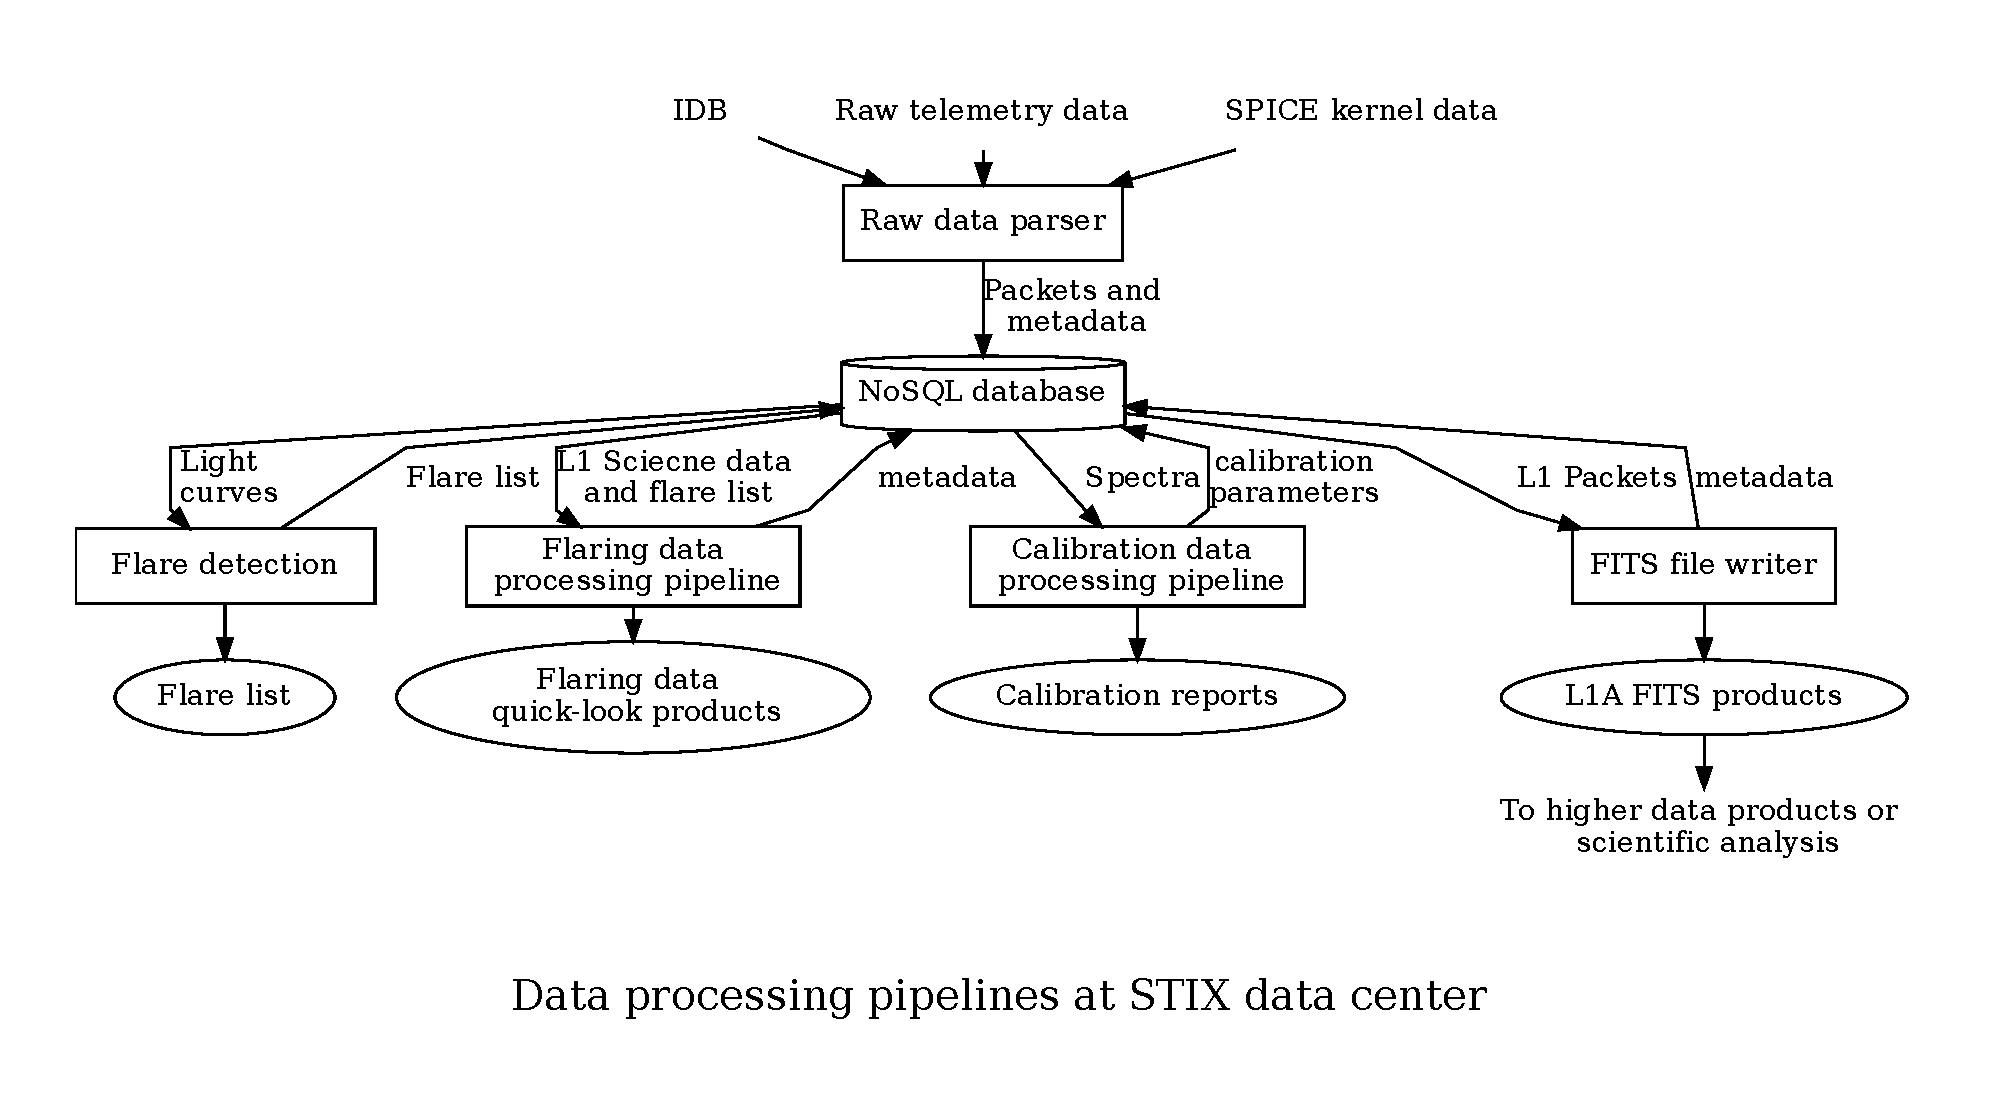
\includegraphics[width=0.9\textwidth]{figures/pipelines.pdf}
    \caption{Data processing pipelines at STIX data center.}
    \label{fig:main_pipelines}
\end{figure*}
New telemetry data arriving at STIX data centers is immediately processed by the pipelines as shown 
in Fig. \ref{fig:main_pipelines}. 
The processing is started from raw packet parsing. Parsed level-1 packets are written to a NoSQL database. 
Then they are selected  are processed in 4 different paths, 
In the first path,  housekeeping, quick-look and science packets 
are selected and used to create L1-A FITS files, 
which can be used for scientific analysis. 
The second path selects calibration data from the database and extracts energy calibration factors for 
instrument monitoring. In the third path, quick-look packets are selected and used to identify solar
flares; The fourth path processes flaring data, 
generating higher data products.   

\subsection{Raw data parsing}
%https://v000658.fhnw.ch/index.php/apps/files/?dir=/Stix/GSW/documents&fileid=1206862
New telemetry data arrived at STIX data center are processed by STIX data parser immediately. 
The parser is capable of decoding all types of STIX binary telecommands and telemetry packets.   
The decoding is based on the mission interface database (MIB), which 
contains information on packet parameters such as names, descriptions, lengths,
data types. Decoded packets contain raw values of parameters. 
 Spacecraft clock times are further converted to UTC times using 
the latest version of SPICE kernel data (\cite{spice1996,spice2018}), compressed integers are  
decompressed by using a LUT table and 
housekeeping raw values are converted to 
human-readable values using the calibration factors or look-up tables stored in the MIB. 
Packets after the above processing steps are called level-1 packets. They
have tree structures, each containing two nodes "header" and "parameters";
the former contains the basic information  of the packet such as timestamp, packet type,
and the latter contains names, 
raw values, engineering values (or decompressed integers) and child nodes of a list of parameters.
Level-1 packets are written 
to a NoSQL database. The NoSQL database is schemaless,  making it ideal to store data with complex
 structures but small sizes like STIX level-1 packets. 

In addition to above processing, the parser also extracts metadata such as data arrival 
times, data acquisition time ranges,  calibration run configuration parameters,  raw data 
filenames. They are written to different collections in the NoSQL database. 
The metadata is necessary for the subsequent processing. 

\subsection{FITS file creation}
After each new raw telemetry file is being parsed, 
housekeeping, quick-look, and science packets  
are selected from the NoSQL database successively 
and checked for data integrity and consistency. 
Then packets of the same type are merged for creations of pre-release of 
level-1 data products (Level-1A)
 in the FITS format (\cite{fits}), 
which is a portable file standard widely used in the astronomy 
community to store images and tables.
Metadata such as observation time range, creation time, filenames,  checksum are written to 
the primary header data units (HDU) of fits files. 
They are also written to a collection in the database.

Level-1A FITS files are generated automatically and available at STIX data center within minutes 
after the reception of a raw file.
It should be noticed that predicted SPICE kernels may be used when the reconstructed spice kernels  
are not available, and the L1A data are subjected to some known issues 
due to bugs in the early version of the flight software.
After all resources are validated,  Level-1  FITS files are created again. 
Level-1  FITS products have almost the same data structures as Level-1A.



\subsection{Energy calibration}
As mentioned earlier, STIX uses 128 Ba$^{133}$ radioactive sources for energy calibration.
The radioactive sources emit  gamma-rays  as they decay, producing prominent photoelectric 
peaks in the calibration spectra (\cite{oliver}). 

The right panel of Fig.\ref{fig:cal-fit} shows 
an example of STIX count spectrum from an in-flight calibration run.  
The three strongest lines are from 31 keV, 35 keV and 81 keV photons. 
The first two peaks are fitted with the double-Gaussian function and the third peak
by the crystall-ball function \cite{crsystallball},  which consists of a Gaussian core portion 
and a power-law low-end tail, below a certain threshold.
Then a linear line is fitted to the relation between
the three fitted peak positions and the photon energies.  
The interception and slope indicate the baseline and gain of the channel. 
The results were compared to the those obtained using the ECC method (see \cite{ecc,ecc2})).
 The results are consistent within errors.
\begin{figure}
 \centering
  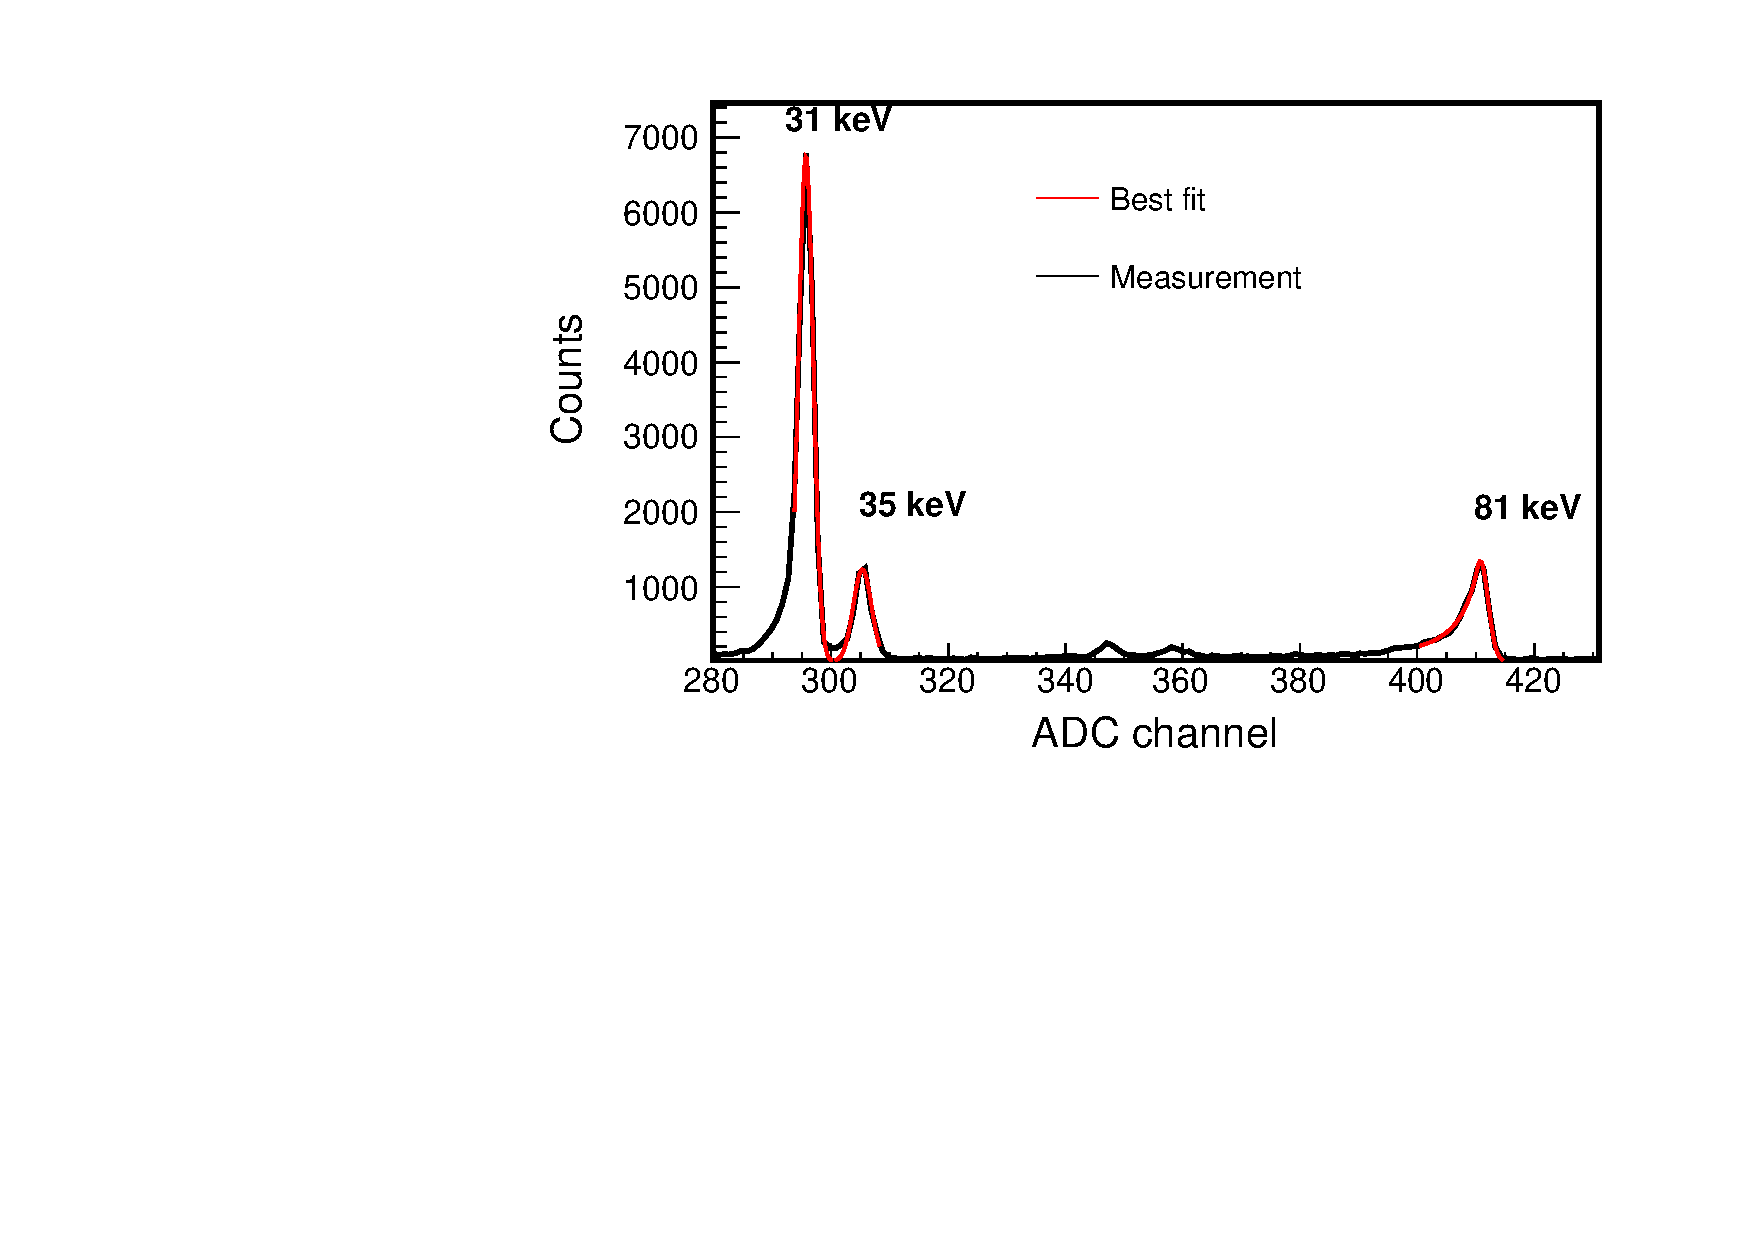
\includegraphics[width=0.8\linewidth]{figures/cal-fit.pdf}
  \caption{ 
   An example of STIX in-flight calibration count spectrum.
  The three strongest lines, from left to right, are from 31 keV, 35 keV, and 81 keV
  photons. The first two peaks are fitted by the double-Gaussian function and the high energy peak by  
  the crystal-ball function. 
}
    \label{fig:cal-fit}
\end{figure}


The above steps are performed for each calibration run automatically 
once the data is available at STIX data center.
Calibration factors obtained the analysis are written to 
the NoSQL database. 
It is accessible through a web page at STIX data center or python APIs.
Once significant differences between the calibration factors and those used to 
construct the onboard energy conversion look-up table (ELUT) are observed, 
a new ELUT is created and commanded to STIX after being validated by STIX operations team. 

\subsection{Solar flare identification}
The in-flight software identifies solar flares by comparing  the count rate of 
the background detector with that of other detectors 
 and packs the results into the QL flare flag and location reports.
However, the reports  only provide limited information on flares due to the constraints of telemetry 
bandwidth and the limitation of onboard computing resources.
Using QL light curves, solar flares can be identified on ground in great detail.


Identification of solar flares on ground is  
triggered after a new QL light curve dataset is available in the NoSQL database. 
QL light curves the energy range from  4 to 10 keV are used for solar flare identification. 
The identification is based on the fact 
that the background event rate in that energy range is almost constant 
over a timescale of days during quiet sun periods. 
The procedure involves the following steps:
\begin{itemize}
  \item Light curve smoothing. The selected light curve is filtered using an unweighted
  moving average filter with a time window of 1 minute to smooth out statistical fluctuations and electric surge spikes;
  \item Identification of flare peaks. Peaks with counts exceeding a threshold of $2\sigma$ above the background level
   are selected. The duration of a peak is given by the time difference between the first 
   crossing of the threshold on the left and right sides of the peak;  
  \item Merging of flare peaks. If the time difference between the two peaks is less than 5 minutes,
   they are considered to be from the same flare.
\end{itemize}

\begin{figure}
  \centering
  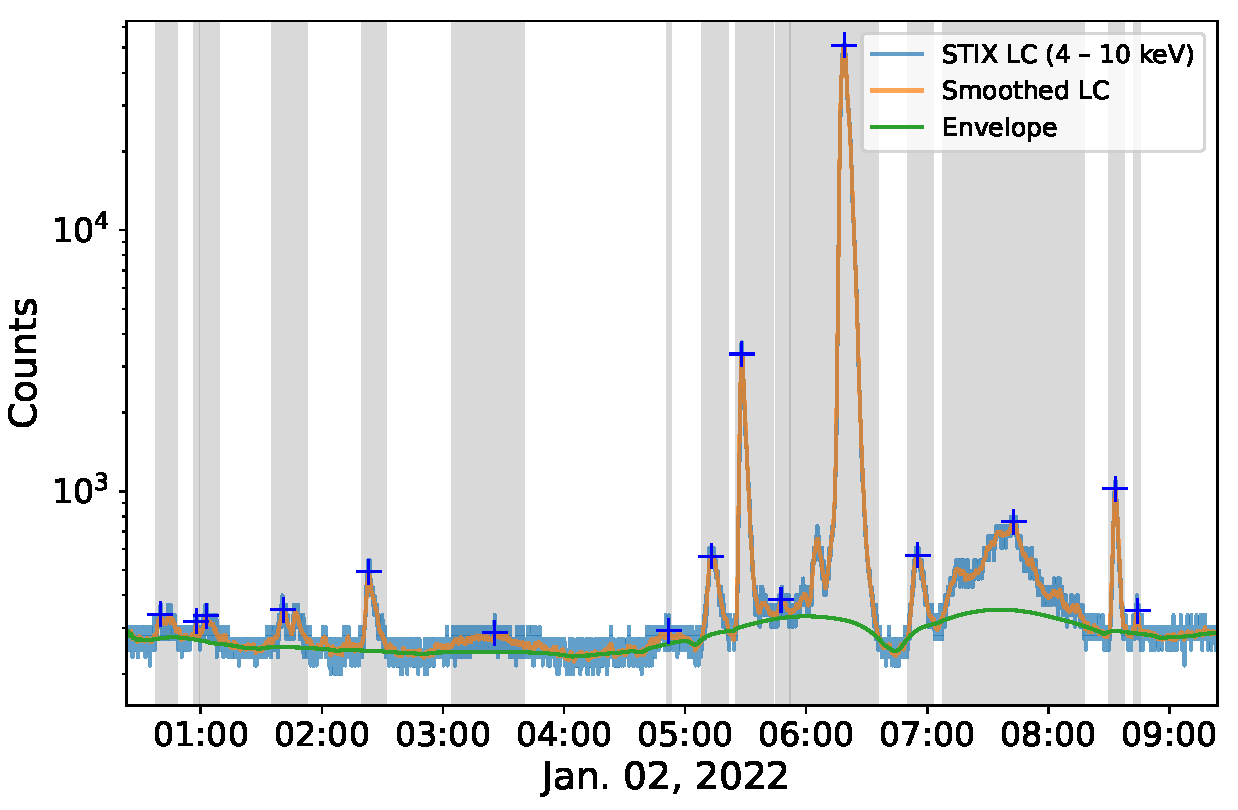
\includegraphics[width=0.8\linewidth]{figures/flaredet.pdf}
  \caption{Solar flares identified from the 4 -- 10 keV QL light curve 
  measured from  2022-02-13T21:00:00Z to 2022-02-14T03:00:00Z. 
  The light curve was smoothed using a moving average filter with a time window
  of 1 minute. Peaks are marked with plus signs and flare time ranges are highlighted in yellow.
  }
  \label{fig:flare-det}
\end{figure}

As an example, Fig.~\ref{fig:flare-det} shows  solar flares  identified from the
4 -- 10 keV QL light curve measured from 2022-02-13T21:00:00Z to 2022-02-14T03:00:00Z, with the procedure above. 
For each identified solar flare, the start time, end time, peak count and  

Before solar flare identification, we select light curves acquired during sun quiet periods to
estimate the background level. The calculated median and root-mean-square of the counts of the five light curves
 are then saved to the database. 
For the identified flares, we will deduct the background we record the width, the time of the peak and the count separately and give each
 flare an identification number. The format of the identification number is an 8-digit number in the format of yyddmmHHMM.
For example, 2201011200 means that the peak time of the flare is UT 2022-01-01T12:00. 
This information is kept in the database.
After completing the flare identification, we exclude the time period of the flare and use the light change curve when no flare occurs as background data,
 repeating the background calculation mentioned earlier, and these data will be used as new data for flare identification.
This list can be accessed using the web page or the api.





\subsubsection{Flare ID naming convention}
\subsubsection{Determination of solar flare GOES classes}

\begin{figure}
  \centering
  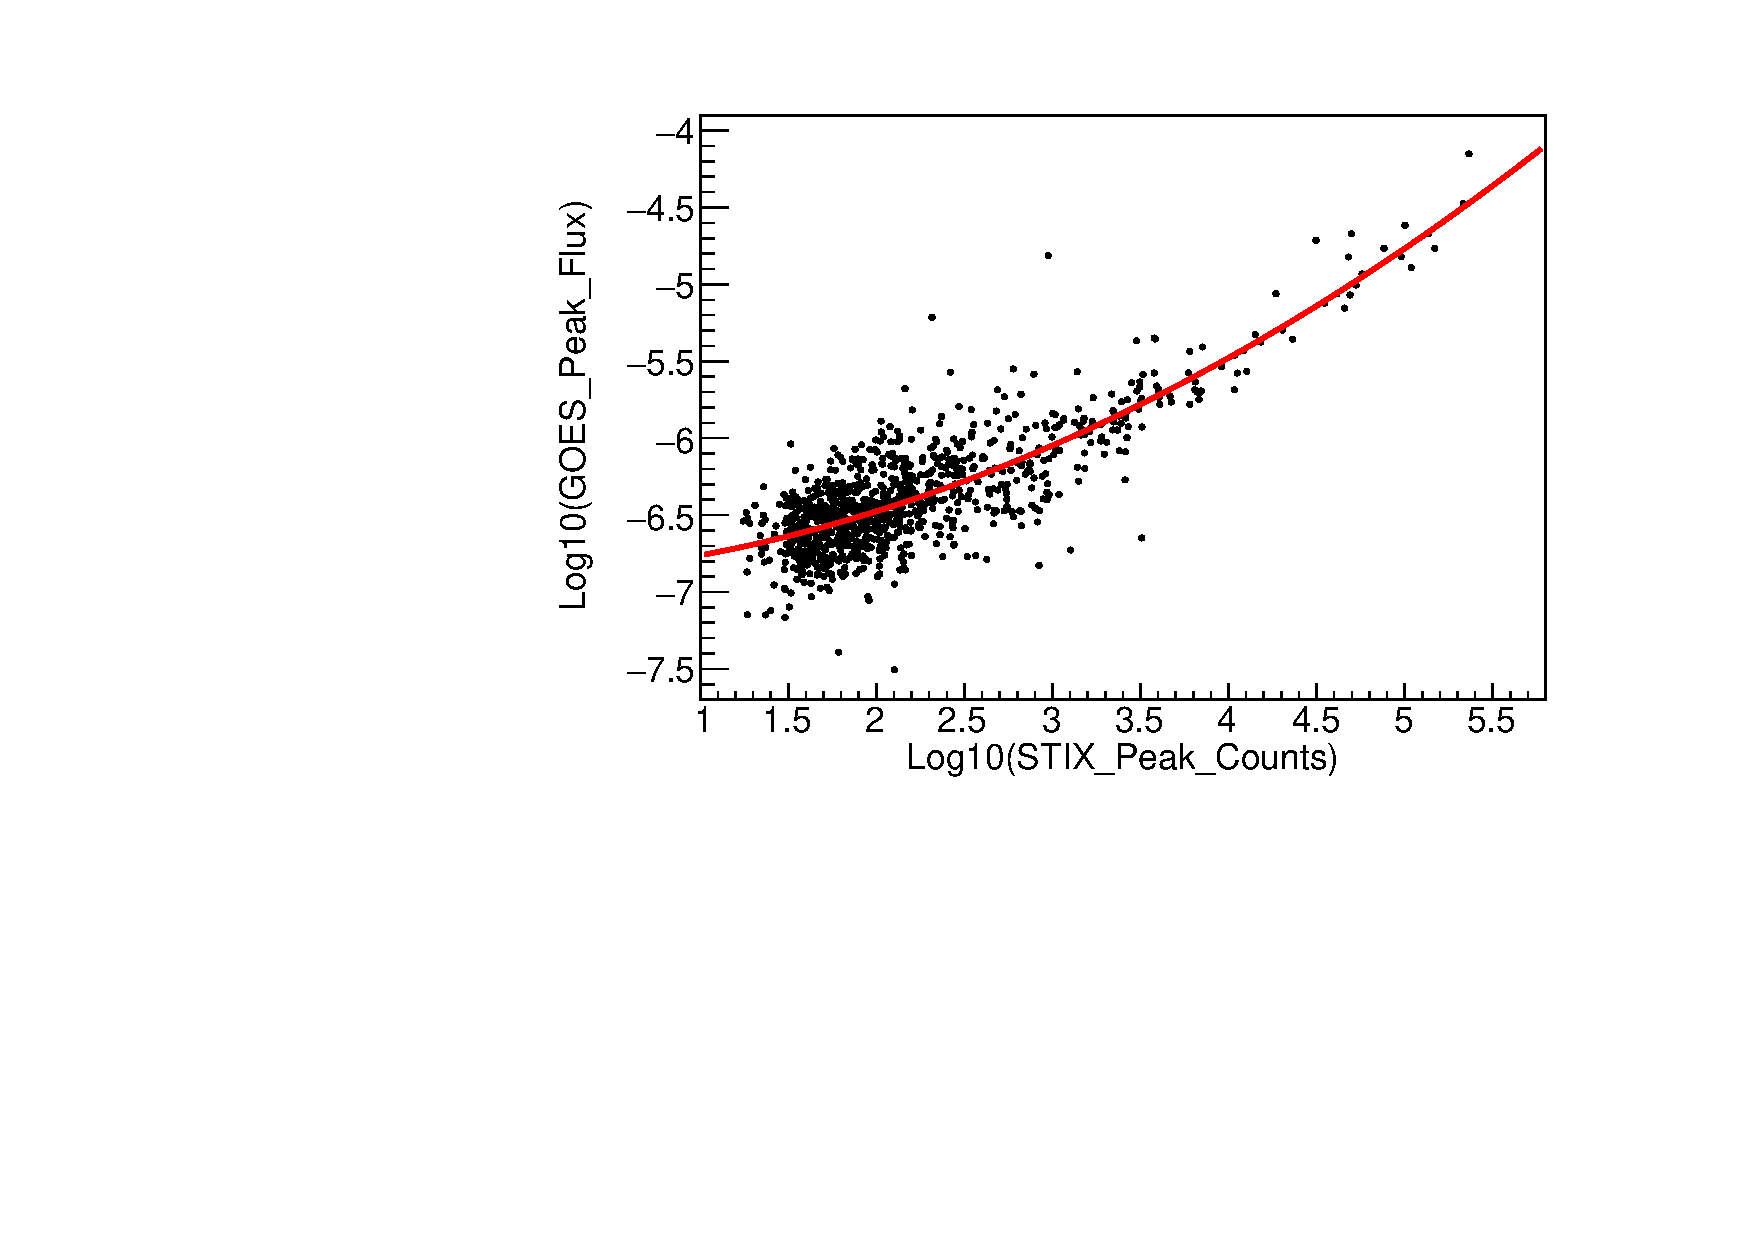
\includegraphics[width=0.8\linewidth]{figures/goes-stix-scatter.pdf}
  \caption{A scatter plot of GOES flux and STIX peak counts in the 4 -- 10 keV quick-look light curve for 989 flares observed by both instruments.
A quadratic function fitted to the log-log data is also shown in the figure. 
STIX counts are background subtracted and 
corrected for flux differences due to the variation of the distance between the Sun and Solar Orbiter. 
The fitted parameters for the quadratic function  are $p_0$=-6.91, $p_1$=0.075 and $p_2$=0.071. 
}
\label{fig:goes-stix}
\end{figure}
For flares that are not observed by GOES. 
A model based on a polynomial fit to the relationship of GOES flux between  STIX counts normalized by the 
squared distance between the Sun and STIX (More details about the model.
Fig. \ref{fig:goes-stix} shows the correlation between GOES flux and STIX peak counts in the 4 -- 10 keV quick-look light curve
for 989 flares observed before Jan. 2022 by both instruments. 
The GOES flux of a solar flare $F$ is estimated using
\begin{equation}
F=10^{p_0+p_1 x+p_2 x^2},
\end{equation}
with
\begin{equation}
 x=\log_{10} {c*r^2}.
\end{equation}
where $p_0$, $p_1$, $p_2$ are the parameters from the curve fit, 
$c$ is STIX background subtracted  counts accumulated in 4 sec and $r$ is 
the distance between the Sun and solar orbiter in units of AU, respectively.
The error of an estimated flux is considered to be the same as the error 
of its nearest data point.

\subsubsection{Flare locations}
STIX uses a dedicated sub-collimator to estimate a rough (within a few arcminutes),
 but unambiguous, flare location on board in near real time.
  The Coarse Flare Locator (CFL) consists of a single grid with
   a specific pattern which selectively illuminates pixels of a 
   dedicated detector based on the source location.
    The correlation between the counts in the pixels of this detector and a look-up table 
    of pre-caculated expectations allows the location to be estimated promptly, 
    within the constraints of on board processing. 
    Using the downloaded measured counts 
    in each pixel the coarse flare location can also be reconstructed on the ground. 
    This allows for more sophisticated algorithms which require greater computational 
    power than is available on board; greater flexibility as to which time and energy 
    intervals are combined; and more careful background subtraction.
\begin{figure*}
  \centering
  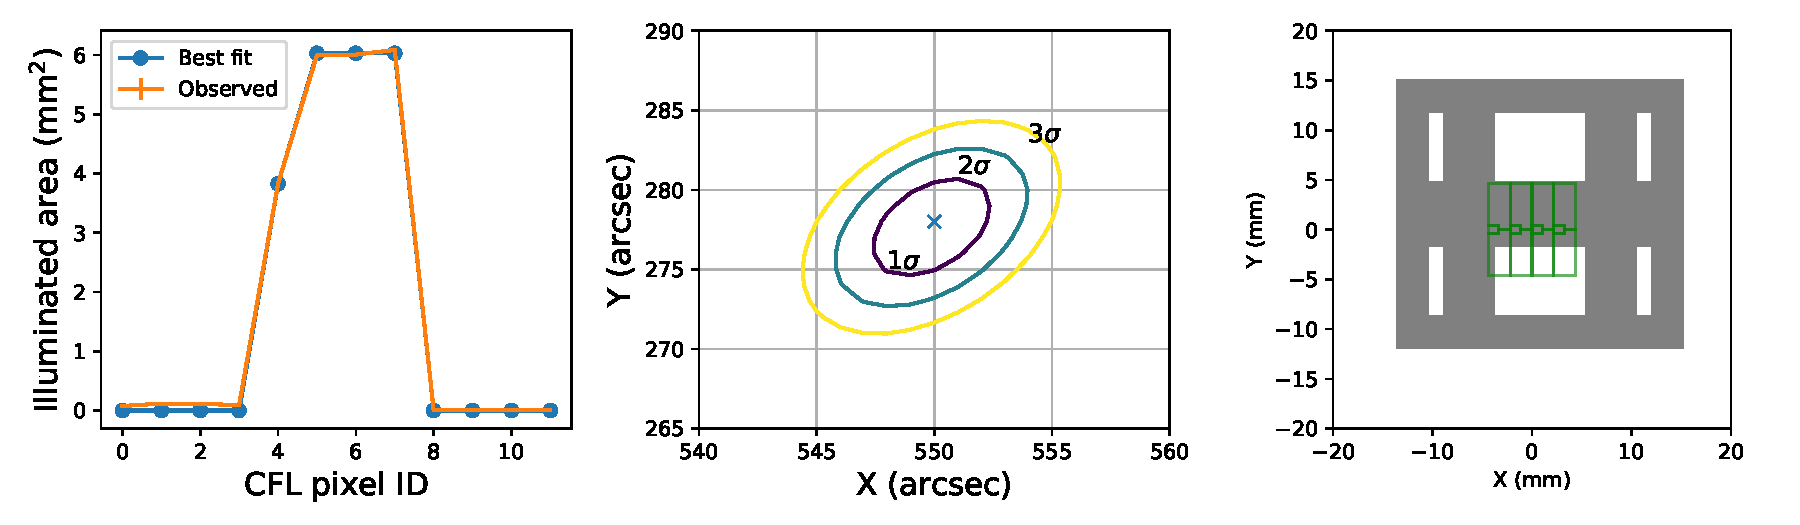
\includegraphics[width=0.95\linewidth]{figures/cflMay07.pdf}
  \caption{Left: area of exposed regions of 12 pixels calculated by combining
  the twelve pixels counts with averages from other detectors, and the best fit.
   Middle: solution of flare location as seen by Solar Orbiter for Flare 202105070034.
   The best fit location is indicated with the symbol X. The 1 $\sigma$, 2 $\sigma$ and 3 $\sigma$ confidence
   regions are also shown. Right: shadow of CFL sub-collimator projected on the twelve CFL pixels.}
  \label{fig:cflpattern}
  %/FHNW/STIX/SolarFlareAnalysis/stix_simulator/cfl
\end{figure*}




\begin{figure*}
  \centering
  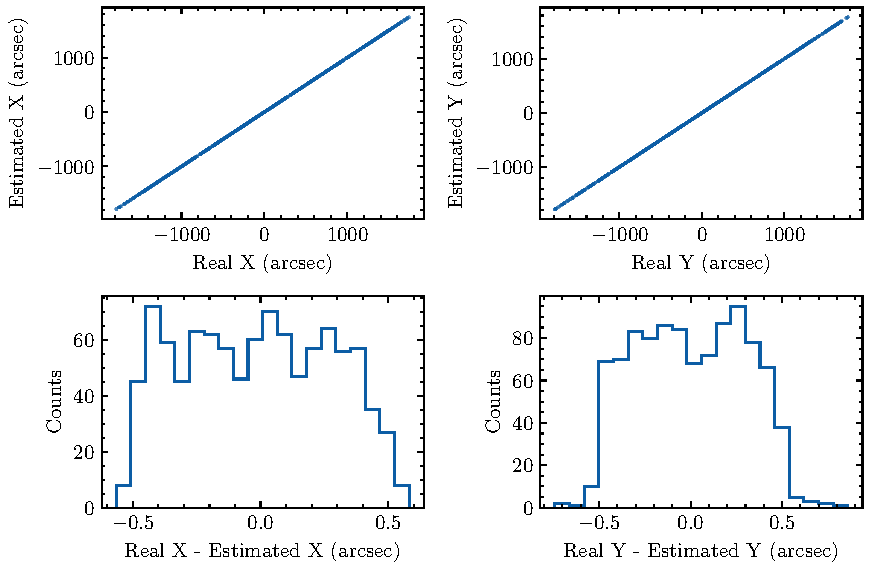
\includegraphics[width=0.7\linewidth]{figures/cflError.pdf}
  \caption{Top: reconstructed coarse flare location solutions against actual locations along the x-axis (left) and y-axis (right). Bottom:
  Differences between the reconstructed and randomly generated locations along
   the x-axis (left) and y-axis (right). The generated sources are assumed to be point-like. Note that statistical
   uncertainties are not considered here. 
    }
  \label{fig:cflerror}
  %/FHNW/STIX/SolarFlareAnalysis/stix_simulator/cfl
\end{figure*}




\subsection{Solar flare list}
\subsection{Flare location database}


A list of products from the flare processing pipeline

* Flare list
* Flare location
*

\subsubsection{Flare location using coarse flare data}
\subsubsection{Flare classification using GOES x-ray flux}

\section{STIX data products}

\subsection{L1 data products}
\begin{itemize}
    \item Raw data.
    \item L1 data.
    \item L2 data
    
\end{itemize}

The latest level 1 FITS IO from Shane has been integrated into the data processing pipeline on pub023 server.

I have recreated fits products for all old telemetry data with the upgraded SW.

The L1 fits files  created by this pipeline have a different data level:  L1A ('A' here means  prerelease/alpha version).

The idea behind L1A data sets is to allow for quicker access to STIX data in the fits format instead of grabbing  data from plots or using JSON requests,

for operations,  debugging  etc.

The L1A data sets can be generated within a few minutes after the arrival of a new raw telemetry file.

The differences between L1A and L1 available in Shane's ftp include:

1.  Two different L1A data files may have duplicated data

2.  L1A data sets are still created for incomplete packets  (L1 checks for data completeness)

3.  SPICE kernel data for telemetry files always arrives  after one or two days later.
    So  there may be a sub-second difference between the UTC time in fits files (same to times on web pages)

   and the real time.

    Shane's formal L1 release can avoid this issue if they are produced on a later date.

4. L1A contains housekeeping data

The different data-processing levels for HMI are summarized as follows, with more details available from this source:
• Data at Level 0 are images that have been constructed from the raw telemetry stream.
• Data at Level 1.0 are images that have been converted from Level 0, with processing including bad-pixel removal, flat-fielding,
and quality assessment checks, but otherwise not having undergone any irreversible data alterations.
• Data at Level 1.5 are images of the physical observables (Dopplergrams, magnetograms, and continuum images), which were
constructed from the individual Level 1.0 filtergrams.
• Data at Level 2 have been irrevocably filtered, time-sequence-merged, Fourier-transformed or otherwise changed from Level 1.5
data in a way that is irreversible. Level 2 products include intermediate products for later production of mission science data
products, such as helioseismic inferences of solar subsurface flows


The Level0 archive contains TM which has been parsed or decommuated into readable structures but no additional external information is include:

times are not converted to UTC
no calibration or conversions applied
for STIX we need to decide if we decompress / combine X-ray L0 the count/trigger data at this stage or in the next level L1

copy manual,
tree like, 
json formats
name, raw value, eng value, children
look-up table, to know description

estimate mongodb benchmark
Mongodb benchmark,
key value, index, performance


\subsection{Auxilary data}



\begin{table}
\centering
\caption{Level 1 data products}
\begin{tabular}{llll}
Category & Type   &  Naming convention  & Remarks   \\ \hline
 Housekeeping & hk\_mini  &  & Houskeeping in BOOT mode   \\
 & hk\_maxi  &  & houskeeping data in NOMINAL   \\
 Quick-look &  light curves &  & Quicklook lightcurves \\
  &  variance &  & variance \\
  &  spectra &  &  \\
  &  background monitor &  &  \\
    &  flare location &  &  \\
 Calibration data &   &  &  \\
\end{tabular}
\end{table}

\section{Data selection and automation}

As the foregoing discussion suggests,
 there are three important distinctions between the 
 QL and primary X-ray data handling: first, the QL data represent only 
 spatially-integrated data;  second, the QL data are acquired and 
 transmitted with fixed parameters such as a 4 s cadence; third, there is no 
 provision for onboard QL data selection. 
In contrast, the much more voluminous primary data can only 
be transmitted on a highly selective (flare-associated) basis, albeit with a wide range of choices for time and energy
 resolution, and coverage. These choices can be optimized to match the dynamic characteristics of the flare in question.  
  Thus by limiting consideration to flare intervals only, and by optimizing time and energy range and 
 resolution for the individual flare, the scientific efficiency of imaging and spectroscopic data telemetry can be greatly enhanced.


There are two approaches to selecting the time- and energy
resolution and range for the bulk spectroscopic and imaging data.
The first approach relies on the ground segment to select param
eters for the downlink of flare T/M. This selection can be based
on the QL light curves in 5 different energy bands which together
provide a robust indication of flare timing, intensity and spectral
properties. The ground segment can use this to choose optimized
time range, energy range, and resolution for different phases of
the flare, predict the resulting T/M volume and upload corresponding analysis requests.
The onboard software then applies
these parameters to the data stored in the archive buffer. This
option is viable because the latency of the QL data (up to 24 h)
is much shorter than the multi-week longevity of the archive
buffer. This provides time for the ground segment to make selections 
and upload parameters and for the FSW to process the data.
Since each ground system requests result in a predictable telemetry volume, 
the STIX ground system is responsible for complying with T/M corridor restrictions on the data rate.

There are three downsides to this approach to data selection:
first, the selections and choices are a labor-intensive activity;
second, selections must be made and satisfied before the onboard
archive is overwritten and so that the choices must be made in a 
timely fashion; third, there is an additional operational latency of
at least a few days between flare occurrence and the transmission
of the requested X-ray imaging and spectroscopic data.
With the second approach (“autonomy”), the FSW uses the
output of the onboard flare detection algorithm to identify rele
vant time ranges. It then uses automatic, parametrized algorithms
to optimize the time and energy resolution for imaging and spec-
troscopic data for inclusion in bulk T/M. As of this writing, this
option has not yet been fully implemented. When using autonomy,
the QL telemetry (Table 3) will include flare and telemetry
management information to show the analysis status of recent
events.

\begin{itemize}
\item L1 request for solar flare.\\
For detected flares,  a script is used to create data requests.
If the background subtracted peak count rate of a flare is greater 150,
both L1 and spectrogram requests are created;  For micro-flares, as only
spectrograms are request normally as the statistics is too
low to reconstruct flare images.  Aspect data requests
and some extra data requests are created for events of interest in the
STIX operations team.
For external users, data request forms can be also submitted using a web tool
at the data center.
\item Spectrogram data requests.
\item Requests for background data
\end{itemize}

An unique ID is assigned to each data request automatically.
The ID naming convention is yyddmmxxxx, in which yyddmm indicate the observation year (without century), month, date,
and the last four digits indicates the serial number of the data request in the day.
IDs are used to track the status of data requests, and reterieve data products from the
STIX data center.
The information of created data requests are stored in the NoSQL database on the same server.
They are converted to instrument operation requests (IORs) after a series of checks.
Requested data will arrive at STIX data center within a time frame of two weeks to three months, depending on
telemetry allocations.

\subsubsection{Background requests}
\subsubsection{data request unique conventions}
\section{Database}
\subsection{Raw data packet database } 
\subsection{Configuration database}
\section{Online data visualization tools}
\subsection{Quick-look light curve}
\subsection{Science data quick analysis}
\subsubsection{Calibration data}

calibration data products
https://fermi.gsfc.nasa.gov/ssc/data/access/gbm/
\subsubsection{Solar Orbiter orbit viewer}
The ISDC maintains a web page through which
data, software, its newletter, general information and links
to other sites are provided. This is accessible through
http://isdc.unige.ch

When a new data file from the platform is received at the PPDC,
it triggers an autonomous start of the dedicated program that decodes and
interprets its contents. The binary data contain the spacecraft location, attitude, speed, and GPS timestamps with increments every half second. The GPS timestamps are converted into Unix-timestamps, where the leap seconds are also considered. After processing, the platform data are written to the ROOT format files. The data start and stop time, data processing time, input filename and ID of the output file of each processing are recorded in a dedicated database table.
SPICE kernel

Updated once per day.

At the center of the Sun.
It is worth mentioning that has to corrected for.
This can be done by using the web tool provided at the auxiliary data center at

\subsection{Automated data request scheme}
scheme

background data request
\subsection{Spectral analysis software}
\subsection{STIX Imagging software}

\section{Data access and APIs}
stixdcpy allows you to query and download data which are available at STIX data center, include
Quick-look light curves
Housekeeping data
Science data
Energy calibration dat which are later included to the low-latency telemetry stream.
Auxilary data
STIX solar flare list



\section{Summary}
\label{sec:summary}



% WARNING
%-------------------------------------------------------------------
% Please note that we have included the references to the file aa.dem in
% order to compile it, but we ask you to:
%
% - use BibTeX with the regular commands:
%   \bibliographystyle{aa} % style aa.bst
%   \bibliography{Yourfile} % your references Yourfile.bib
%
% - join the .bib files when you upload your source files
%-------------------------------------------------------------------

\bibliographystyle{aa}
\bibliography{citations}

\end{document}
